\documentclass[10.5pt,scale=1.0,t,aspectratio=169,hyperref={pdfpagelabels=false}]{beamer}


\usepackage{lipsum}
\usepackage{color}
\usepackage{amsfonts}
\usepackage{amsmath,mathtools}
\usepackage{mathrsfs}
\usepackage{array}
\usepackage{algorithm}
\usepackage{hyperref}
\usepackage[spanish,es-nodecimaldot]{babel}
\usepackage[utf8]{inputenc}
\usepackage{graphicx}
\usepackage{multicol}
\usepackage{multirow}
\usepackage{enumitem}
\usepackage[document]{ragged2e}
\usepackage[absolute,overlay]{textpos}
\textblockorigin{0mm}{0mm} 
\usefonttheme[onlymath]{serif}
\usepackage{verbatim}
\usepackage{cite}




\newenvironment{conditions}[1][where:]
{#1 \begin{tabular}[t]{>{$}l<{$} @{${}={}$} l}}
	{\end{tabular}\\[\belowdisplayskip]}


\newcolumntype{L}{>{$}l<{$}} % math-mode version of "l" column type


\newcounter{saveenumi}
\newcommand{\seti}{\setcounter{saveenumi}{\value{enumi}}}
\newcommand{\conti}{\setcounter{enumi}{\value{saveenumi}}}

\setbeamertemplate{bibliography item}{\insertbiblabel}


\hypersetup{colorlinks=true,
	linkcolor=blue,
	linktoc=all,				
	citecolor=blue,
	urlcolor=red,
	pdftitle={ELECTRONICA DIGITAL},
	pdfauthor={Santiago Rúa Pérez},
	pdfcreator={Santiago Rúa Pérez}}


\definecolor{GreenDark}{rgb}{0.0, 0.60, 0.0}
\definecolor{RedDark}{rgb}{183, 0.0, 0.0}
\definecolor{BlueDark}{rgb}{0.0, 0.0, 167}
\definecolor{BlueLight}{rgb}{0.2, 0.451, 0.517}


\graphicspath{{imag/}}

\newcommand{\Ho}{$H_{0}$}
\newcommand{\Ha}{$H_{a}$}
\newcommand{\Nota}{{\bf Nota: }}
\newcolumntype{P}[1]{>{\centering\arraybackslash}p{#1}}
\newcolumntype{M}[1]{>{\centering\arraybackslash}m{#1}}

\newcommand{\less}{<}
\newcommand{\greater}{>}


\setlength{\parindent}{1em}
\setlength{\parskip}{.6em}
\renewcommand{\baselinestretch}{.9}

%%%%    C environment    ---------------- %%%%%%%%%%%%%%%.
\usepackage{listings}
\usepackage{xcolor}
\definecolor{mGreen}{rgb}{0,0.6,0}
\definecolor{mGray}{rgb}{0.5,0.5,0.5}
\definecolor{mPurple}{rgb}{0.58,0,0.82}
\definecolor{backgroundColour}{rgb}{0.95,0.95,0.92}

\lstdefinestyle{CStyle}{
	backgroundcolor=\color{backgroundColour},   
	commentstyle=\color{mGreen},
	keywordstyle=\color{magenta},
	numberstyle=\tiny\color{mGray},
	stringstyle=\color{mPurple},
	basicstyle=\scriptsize,
	breakatwhitespace=false,         
	breaklines=true,                 
	captionpos=b,                    
	keepspaces=true,                 
	numbers=left,                    
	numbersep=5pt,                  
	showspaces=false,                
	showstringspaces=false,
	showtabs=false,                  
	tabsize=2,
	language=C
}
%%--------------------------------------------------------------------------


\title{Electrónica Digital II}   
\author{Santiago Rúa Pérez, PhD.} 
\date{\today} 

\setlength{\TPHorizModule}{\textwidth}
\setlength{\TPVertModule}{\textwidth}

\newcommand{\btVFill}{\vskip0pt plus 1filll}


\setbeamertemplate{sidebar right}{}
\setbeamertemplate{footline}
{
	\leavevmode%
	\hbox{%
		\begin{beamercolorbox}[wd=.333333\paperwidth,ht=2.25ex,dp=1ex,center]{author in head/foot}%
			\usebeamerfont{author in head/foot}\insertshortauthor
		\end{beamercolorbox}%
		\begin{beamercolorbox}[wd=.333333\paperwidth,ht=2.25ex,dp=1ex,center]{title in head/foot}%
			\usebeamerfont{title in head/foot}\insertshorttitle
	\end{beamercolorbox}}%
	\vskip0pt%
}
\makeatother

\begin{document}
	%%%%%%%%%%%%%%%%%% FRAME %%%%%%%%%%%%%%%%%%%%%%%%%%
	\begin{frame}
		\titlepage
	\end{frame}
	%%%%%%%%%%%%%%%%% FRAME START %%%%%%%%%%%%%%%%%%%%%%%%%%
	\frame{
		%\frametitle{}
		\begin{center}
			\LARGE \textcolor{blue}{UNIONES, ESTRUCTURAS Y MANIPULACIÓN DE BITS EN C}
		\end{center}
		
	}

%%%%%%%%%%%%%%%%% FRAME %%%%%%%%%%%%%%%%%%%%%%%%%%
\frame{
\frametitle{Estructuras, Uniones y Manipulación de bits en C}
{\bf Objetivos}
\begin{itemize}
\item Crear y usar estructuras, uniones y enumeraciones.
\item Entender la auto referenciación de las estructuras.
\item Como operar con estructuras.
\item Inicilizar estructuras.
\item Usar typedef.
\item Usar constantes enum.
\item Manipulación de bits. 
\end{itemize}
}
%%%%%%%%%%%%%%%%% FRAME %%%%%%%%%%%%%%%%%%%%%%%%%%
\begin{frame}[fragile]
\frametitle{Estructuras en C}
	En C, las estructuras son tipos de datos agrupados bajo un mismo elemento. El objetivo es formar una variable nueva conformada por diferentes tipos. 
	\begin{lstlisting}[style=CStyle]
		struct employee{
			char firstName[20];
			char lastName[20];
			unsigned int age;
			char gender;
			double hourlySalary;
		}
	\end{lstlisting}
	La referenciación a si mismo dentro de una estructura puede darse siempre y cuando se utilicen punteros. 
	
	\begin{lstlisting}[style=CStyle]
		struct employee{
			char firstName[20];
			struct employee *teamLeaderPtr; // pointer
		}
	\end{lstlisting}

	Este tipo de autollamado permite construir elementos mas complejos como listas enlazadas (\textit{linked list})
\end{frame}

%%%%%%%%%%%%%%%%% FRAME %%%%%%%%%%%%%%%%%%%%%%%%%%
\begin{frame}[fragile]
	\frametitle{Inicializaci\'on y acceso a estructuras}
	Se define la estructura con el identificador y el nombre de la estructura. En el ejemplo se declara un variable aCard, un arreglo de estructuras deck y un puntero a dicha estructura.
	\begin{lstlisting}[style=CStyle]
		struct card aCard, deck[52], *cardPtr;
	\end{lstlisting}
	\begin{itemize}
		\item No estan almacenados en espacios continuos de memoria. 
		\item Se pueden inicializar utilizando una lista de elementos en el orden de la definici\'on.
		\begin{lstlisting}[style=CStyle]
			struct card aCard = { "Three", "Hearts" };
		\end{lstlisting}
		\item Se accede a miembros de la estructura usando $\cdot$ o $->$ cuando se tiene una variable o un puntero respectivamente.
		\begin{lstlisting}[style=CStyle]
			printf("%s", aCard.suit); // displays Hearts
			printf("%s", cardPtr->suit); // displays Hearts
		\end{lstlisting}
		\item Las estructuras pueden ser pasadas valores individuales o puntero a la estructura.
	\end{itemize}
\end{frame}

%%%%%%%%%%%%%%%%% FRAME %%%%%%%%%%%%%%%%%%%%%%%%%%
\begin{frame}[fragile]
	\frametitle{Estructuras en C}
	\textcolor{blue}{Ejemplo}
	
	\begin{lstlisting}[style=CStyle]
		#include<stdio.h>
		struct  card
		{
			char *face;
			char *suit;
		};
		int main(void){
			struct card aCard;
			aCard.face = "Ace";
			aCard.suit = "Spades";
			struct card *cardPtr = &aCard;
			
			printf("%s%s%s\n%s%s%s\n%s%s%s\n", aCard.face, " of ", aCard.suit,
			cardPtr->face, " of ", cardPtr->suit,
			(*cardPtr).face, " of ", (*cardPtr).suit);
			
		}
	\end{lstlisting}

	Las estructura pueden pasarse a funciones completamente o valores de la estructura. Tambien paso por referencia. 
\end{frame}


%%%%%%%%%%%%%%%%% FRAME %%%%%%%%%%%%%%%%%%%%%%%%%%
\begin{frame}[fragile]
	\frametitle{Typedef en C}
	La palabra \texttt{typedef} sirve como mecanismo para crear sinónimos de variables previamente definidas. 
	
	\begin{lstlisting}[style=CStyle]
		typedef struct {
			char *face;
			char *suit;
		}Card;
	\end{lstlisting}
	
	Una vez declarada el tipo de datos Card, ahora se puede utilizar para crear una variable.
	
	\begin{lstlisting}[style=CStyle]
		Card deck[52]
	\end{lstlisting}
\end{frame}

%%%%%%%%%%%%%%%%% FRAME %%%%%%%%%%%%%%%%%%%%%%%%%%
\begin{frame}[fragile]
	\frametitle{Typedef en C - Ejemplo}
	\vspace{-0.2in}
	\begin{multicols}{2}
		\begin{lstlisting}[style=CStyle,basicstyle=\tiny]
#include <stdio.h>
#include <stdlib.h>
#include <time.h>

#define CARDS 52
#define FACES 13

struct card {
	const char *face; // define pointer face
	const char *suit; // define pointer suit
};
typedef struct card Card; // new type name 

void fillDeck(Card * const wDeck, const char * wFace[], const char * wSuit[]);
void shuffle(Card * const wDeck);
void deal(const Card * const wDeck);

int main(void)
{
	Card deck[CARDS]; // define array of Cards
	
	const char *face[] = { "Ace", "Deuce", "Three", "Four", "Five", "Six", "Seven", "Eight", "Nine", "Ten","Jack", "Queen", "King"};
	const char *suit[] = { "Hearts", "Diamonds", "Clubs", "Spades"};
	
	srand(time(NULL)); // randomize
	fillDeck(deck, face, suit); // load the deck
	shuffle(deck); // put Cards in random order
	deal(deck); // deal all 52 Cards
}

void fillDeck(Card * const wDeck , const char * wFace[], const char * wSuit[])
{
	for (size_t i = 0; i < CARDS; ++i) {
		wDeck[i].face = wFace[i % FACES];
		wDeck[i].suit = wSuit[i / FACES];
	}
}

void shuffle(Card * const wDeck)
{
	for (size_t i = 0; i < CARDS; ++i) {
		size_t j = rand() % CARDS;
		Card temp = wDeck[i];
		wDeck[i] = wDeck[j];
		wDeck[j] = temp;
	}
}

void deal(const Card * const wDeck )
{
	for (size_t i = 0; i < CARDS; ++i) {
		printf("% 5s of %-8s% s",wDeck[i].face, wDeck[i].suit , (i + 1) % 4 ? " " : "\n");
	}
}
		\end{lstlisting}
	\end{multicols}
	
\end{frame}

%%%%%%%%%%%%%%%%% FRAME %%%%%%%%%%%%%%%%%%%%%%%%%%
\begin{frame}[fragile]
	\frametitle{Uniones en C}
	Las uniones son tipos de datos derivados los cuales comparten el mismo espacio de memoria. Define un tipo de variable con diferentes connotaciones. Solo puede tener un valor al tiempo. 
	
	\begin{lstlisting}[style=CStyle,basicstyle=\tiny]
		#include <stdio.h>
		union number {
			int x;
			double y;
		};
		int main(void)
		{
			union number value; 
			value.x = 100; // put an integer
			
			printf("% s\n% s\n% s\n % d\n\n% s\n % f\n\n\n",
			"Put 100 in the integer member",
			"and print both members.",
			"int:", value.x,
			"double:", value.y);
			
			
			value.y = 100.0; // put a double 
			printf("% s\n% s\n% s\n % d\n\n% s\n % f\n",
			"Put 100.0 in the floating member",
			"and print both members.",
			"int:", value.x,
			"double:", value.y);
		}
	\end{lstlisting}
\end{frame}
%%%%%%%%%%%%%%%%% FRAME %%%%%%%%%%%%%%%%%%%%%%%%%%
\begin{frame}
	\frametitle{Operadores bit a bit}
	Son operadores que trabajan a nivel de bits en las estructura de datos. 
	\begin{figure}
		\centering
		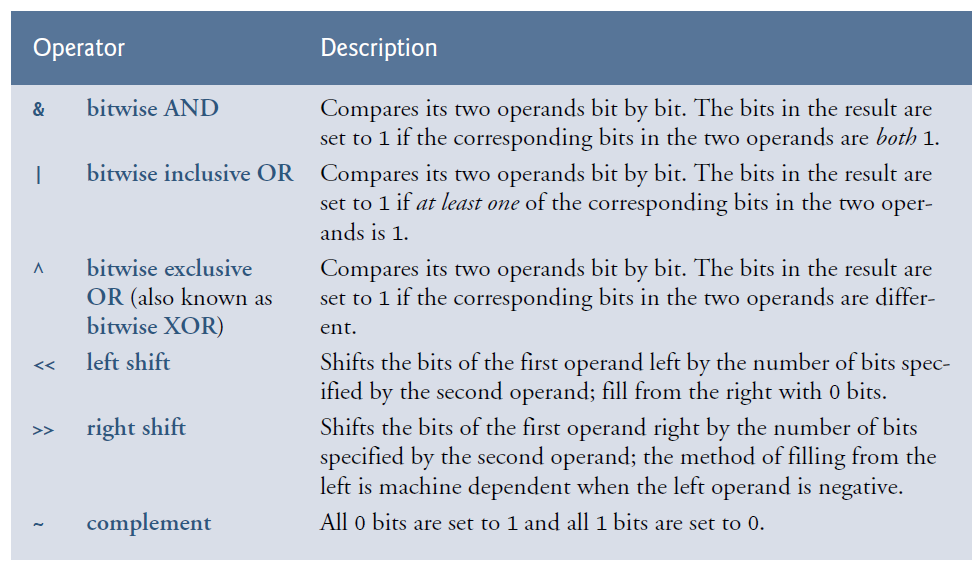
\includegraphics[scale=0.6]{Bitwise}
	\end{figure}
\end{frame}
%%%%%%%%%%%%%%%%% FRAME %%%%%%%%%%%%%%%%%%%%%%%%%%
\begin{frame}[fragile]
	\frametitle{Operadores bit a bit - Ejemplo}
		\begin{lstlisting}[style=CStyle,basicstyle=\tiny]
			#include <stdio.h>
			
			void displayBits(unsigned int value); // prototype
			
			int main(void)
			{
				unsigned int x; // variable to hold user input
				
				printf("% s", "Enter a nonnegative int: ");
				scanf("% u", &x);
				
				displayBits(x);
			}
			
			void displayBits(unsigned int value)
			{
				// define displayMask and left shift 31 bits
				unsigned int displayMask = 1 << 31;
				printf("%10u = ", value);
				
				// loop through bits
				for (unsigned int c = 1; c <= 32; ++c) {
					putchar(value & displayMask ? '1' : '0');
					value <<= 1; // shift value left by 1
					if (c % 8 == 0) { // output space after 8 bits
					putchar(' ');
				}
			}
			putchar('\n');
		}
		\end{lstlisting}
\end{frame}
%%%%%%%%%%%%%%%%% FRAME %%%%%%%%%%%%%%%%%%%%%%%%%%
\begin{frame}[fragile]
	\frametitle{Campos de bit (Bit fields)}
	En C se puede especificar la cantidad de bits a utilizar para almacenar un miembro en una estructura. Estos solo pueden ser declarados en enteros o enteros no signados. 
	\begin{lstlisting}[style=CStyle,basicstyle=\tiny]
		struct bitCard {
			unsigned int face : 4;
			unsigned int suit : 2;
			unsigned int color : 1;
		};
	\end{lstlisting}	
	Es posible especificar un campo de bits sin nombre con el objetivo que se bloquee dicho espacio en memoria.
	\begin{lstlisting}[style=CStyle,basicstyle=\tiny]
		struct example {
			unsigned int a : 13;
			unsigned int   : 19;
			unsigned int b : 4;
		};
	\end{lstlisting}
	Tambien puede ser de tama\~no cero para alinear el siguiente campo con la memoria.
\end{frame}
%%%%%%%%%%%%%%%%% FRAME %%%%%%%%%%%%%%%%%%%%%%%%%%
\begin{frame}[fragile]
	\frametitle{Enumeración}
	Es un conjunto de n\'umeros enteros representados por algun identificador. Comienzan en cero e incrementan de a uno, a no ser que se indique o inicialice de otra forma. 
	\begin{lstlisting}[style=CStyle,basicstyle=\tiny]
	#include <stdio.h>
	
	enum months {
		JAN = 1, FEB, MAR, APR, MAY, JUN, JUL, AUG, SEP, OCT, NOV, DEC
	};
	
	int main(void)
	{
		// initialize array of pointers
		const char *monthName[] = { "", "January", "February", "March",
			"April", "May", "June", "July", "August", "September", "October",
			"November", "December" };
		
		// loop through months
		for (enum months month = JAN; month <= DEC ; ++month) {
			printf("%2d%11s\n", month, monthName[month]);
		}
	}
	\end{lstlisting}
\end{frame}

%%%%%%%%%%%%%%%%% FRAME %%%%%%%%%%%%%%%%%%%%%%%%%%
\begin{frame}
	\frametitle{Ejercicios}
	Encuentre el error
	\begin{figure}
		\centering
		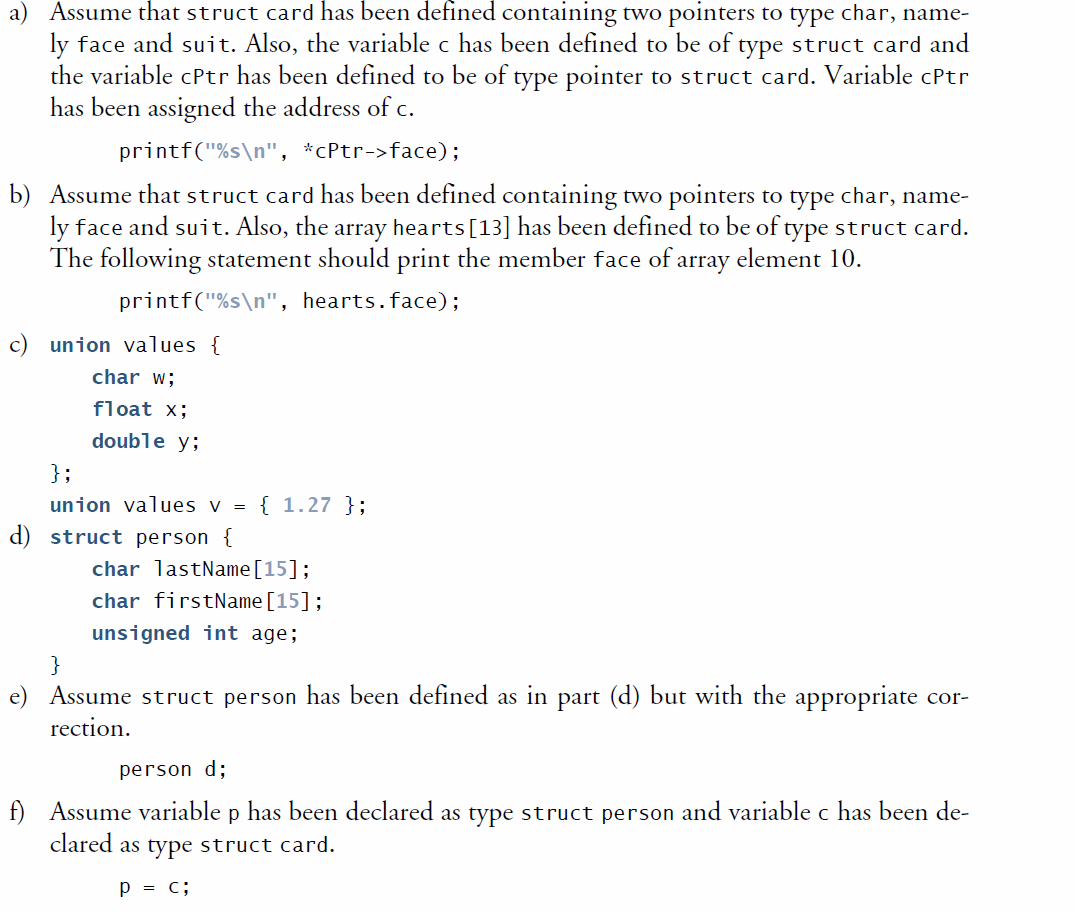
\includegraphics[scale=0.45]{ErrorUnion}
	\end{figure}
\end{frame}
%%%%%%%%%%%%%%%%% FRAME %%%%%%%%%%%%%%%%%%%%%%%%%%
\begin{frame}
	\frametitle{Ejercicios}
	\begin{itemize}
		\item Escribe un programa que invierta el orden de los bits en un dato entero no signado. El programa debe ingresar el valor del usuario y llamar a la función reverseBits	para imprimir los bits en orden inverso. Imprima el valor en bits antes y después de que los bits sean invertido para confirmar que los bits se invierten correctamente.
		\item Crear una union floatingPoint con miembros float f, double d y long
		double x. Escriba un programa que ingrese valores de tipo float, double y long double y almacene el valor en variables de unión de tipo union floatingPoint. Cada variable de unión debe imprimirse como un flotador, un doble y un doble largo. ¿Los valores siempre se imprimen correctamente?
		\item Investigue el algoritmo de barajado de Fisher-Yates en línea,
		luego úsalo para reimplementar el método aleatorio		
	\end{itemize}
\end{frame}
%%%%%%%%%%%%%%%%% FRAME %%%%%%%%%%%%%%%%%%%%%%%%%%
\frame{
\begin{center}
	\LARGE \textcolor{blue}{UNIONES, ESTRUCTURAS Y MANIPULACION DE BITS EN C}
\end{center}

\begin{center}
	\LARGE \textcolor{blue}{GRACIAS}
\end{center}
}

%%%%%%%%%%%%%%%%%%%%%%%%%%%%%%%%%%%%%%%%%%%%%%%%%%%%%%%%%%%%%%%%%%%%%%%%%%%%%%%%%%%%%%%%%%%%%%%%%%%%%%%%%%%%%



\end{document}

